\section{Evaluation}

Correctness is validated end to end. The compiled and simulated output of the
LeNet model is compared against \texttt{onnxruntime} on a seeded random input; the
maximum absolute difference is at the level of fp32 rounding, on the order of
$10^{-8}$, at every optimization level and both under a generous budget and under
a tight budget that forces spilling. The benchmark harness records one result per
cell, each carrying a manifest of the git revision, the LLVM tag \LlvmTag, the
tool versions, and the cost model constants, so every number below traces to a
recorded experiment. Table~\ref{tab:results} is generated from those files.

\begin{table}[h]
  \centering
  \begin{tabular}{llrrrrr}
\toprule
Model & O & Budget (KB) & Instrs & Cycles & DRAM (KB) & Max error \\
\midrule
lenet & 0 & 140 & 91 & 23421 & 339.3 & 3.0e-08 \\
lenet & 1 & 140 & 94 & 33834 & 502.0 & 3.0e-08 \\
lenet & 2 & 140 & 86 & 33930 & 508.1 & 3.0e-08 \\
lenet & 0 & 1024 & 91 & 23421 & 339.3 & 3.0e-08 \\
lenet & 1 & 1024 & 82 & 13008 & 176.6 & 3.0e-08 \\
lenet & 2 & 1024 & 70 & 12710 & 176.6 & 3.0e-08 \\
\bottomrule
\end{tabular}

  \caption{Per cell results: instruction count, simulated cycles, total DRAM
    traffic, and maximum absolute error against onnxruntime. Cycle and DRAM
    figures are simulated estimates.}
  \label{tab:results}
\end{table}

\begin{figure}[h]
  \centering
  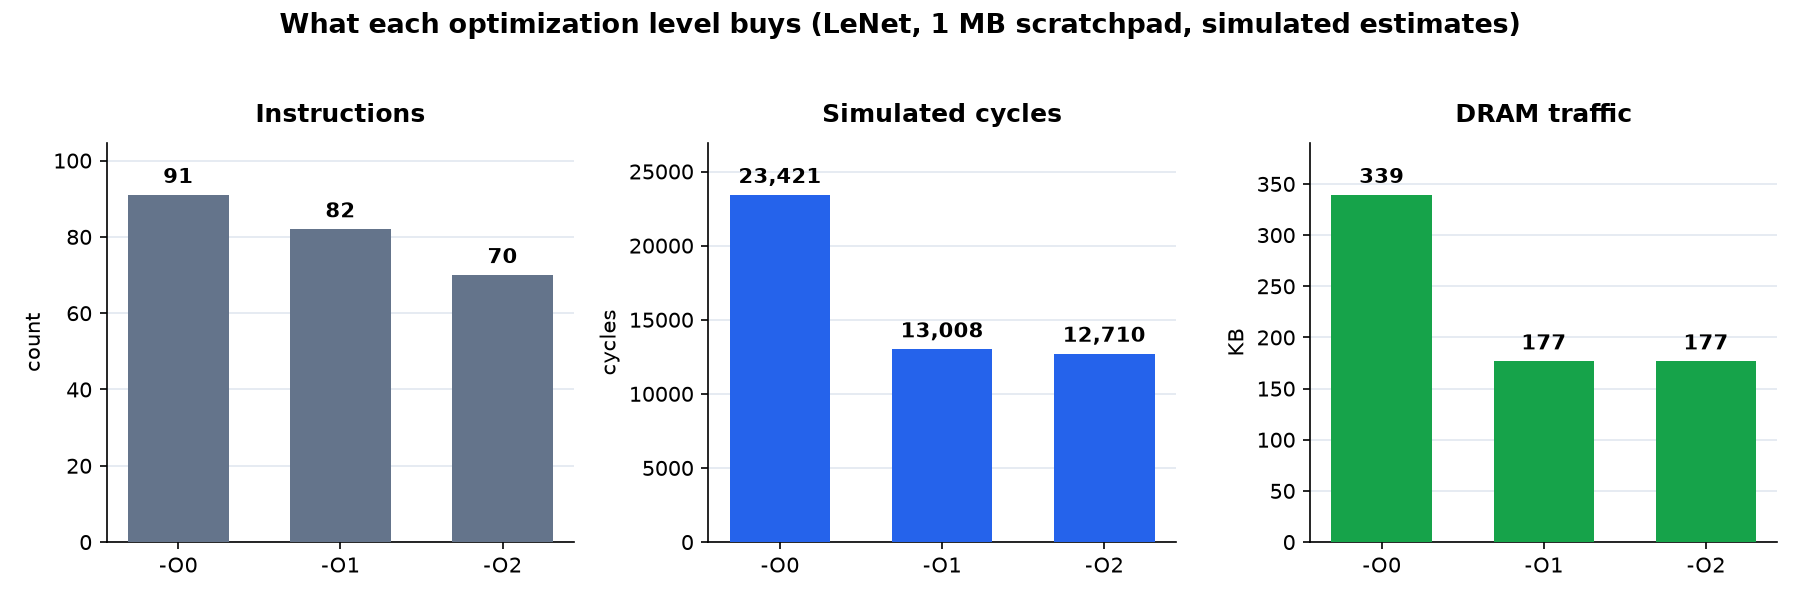
\includegraphics[width=\textwidth]{../docs/images/optimization_levels}
  \caption{What each optimization level buys on LeNet at the one megabyte budget:
    instruction count, simulated cycles, and DRAM traffic all fall from
    \texttt{-O0} to \texttt{-O2}, while the numerics stay exact. Simulated
    estimates.}
  \label{fig:levels}
\end{figure}

Two effects stand out at the one megabyte budget, where nothing spills. Moving
from \texttt{-O0} to \texttt{-O1}, canonicalization and dead code elimination
remove the transposed Gemm weight constants that the importer leaves behind, and
the total DRAM traffic falls from \OaDram{} KB to \ObDram{} KB. Moving to
\texttt{-O2}, fusion folds the four activations into their producers, and the
instruction count falls from \OaInstr{} to \OcInstr{} while the simulated cycles
fall from \OaCycles{} to \OcCycles{}.

\subsection{What each pass buys, one at a time}

The level comparison above says what \texttt{-O2} buys over \texttt{-O0}. It
cannot say what any single pass buys, because the levels are cumulative. Table
\ref{tab:ablation} answers that directly: each row is the full \texttt{-O2}
pipeline with one pass removed, compiled, encoded, simulated, and checked
against onnxruntime exactly as a normal cell is. The deltas are ablated minus
full \texttt{-O2}, so a positive number is what removing the pass costs, which
is the pass earning its place.

\begin{table}[h]
  \centering
  \begin{tabular}{llrrrrr}
\toprule
Budget & Pass removed & Instrs & $\Delta$ & Cycles & $\Delta$ & $\Delta$ DRAM (KB) \\
\midrule
1024 KB & \texttt{canonicalize} & 21 & +0 & 12710 & +0 & +0.0 \\
1024 KB & \texttt{npu-fuse-ops} & 25 & +4 & 13008 & +298 & +0.0 \\
1024 KB & \texttt{symbol-dce} & 21 & +0 & 12710 & +0 & +0.0 \\
140 KB & \texttt{canonicalize} & 29 & +0 & 33930 & +0 & +0.0 \\
140 KB & \texttt{npu-fuse-ops} & 31 & +2 & 33834 & -96 & -6.1 \\
140 KB & \texttt{symbol-dce} & 29 & +0 & 33930 & +0 & +0.0 \\
\bottomrule
\end{tabular}

  \caption{Leave one out ablation of every \texttt{-O2} pass, at both scratchpad
  budgets. Instructions, cycles, and DRAM are simulated estimates from the
  analytical cost model, not measurements. Deltas are the ablated pipeline minus
  full \texttt{-O2} at the same budget, so a positive delta means removing the
  pass made the program worse. \texttt{canonicalize} is ablated everywhere it
  appears, which is twice in the \texttt{-O2} pipeline.}
  \label{tab:ablation}
\end{table}

At the generous budget only one pass buys anything: \BestPass{} is worth
\BestPassCycles{} simulated cycles and \BestPassInstrs{} instructions, and
removing either \texttt{canonicalize} or \texttt{symbol-dce} produces a byte
identical program. That is not a measurement error. \texttt{-npu-fuse-ops}
drives its patterns with a greedy rewriter whose fixed point loop folds
constants and removes dead operations as a side effect, so on this model it
subsumes everything canonicalization had to contribute. Canonicalization still
matters at \texttt{-O1}, where it is the only pass and is responsible for the
whole drop from \OaDram{} KB to \ObDram{} KB; it is redundant only in the
presence of fusion. This is exactly the interaction a leave one out ablation
exposes and a per pass measurement cannot, since measured in isolation
canonicalization does remove operations.

The tight budget reverses the sign. Removing \BestPass{} there changes the
simulated cycles by \BestPassTightCycles{} and the DRAM traffic by
\BestPassTightDram{} KB, both of which are improvements: fusion makes the
program worse when the scratchpad cannot hold the working set. Fusing an
activation into its producer extends that value's live range, and under a budget
that already forces spilling, a longer live range costs a spill and its reload.
A table reporting only the generous budget would have shown fusion as the one
pass worth having and missed that it is counterproductive under pressure.

The tight budget rows show the memory model at work. When the scratchpad cannot
hold the working set, the allocator spills buffers to DRAM and reloads them, which
raises the instruction count and the DRAM traffic relative to the generous budget.
The numerics are unchanged, because a spill is a value preserving round trip.
Finding and fixing a bug in that round trip, where spill temporaries were not
being given distinct DRAM addresses, is one of the cases the benchmark suite
caught and the debug report discusses.
